% !TEX TS-program = pdflatex
% !TEX encoding = UTF-8 Unicode

% Matthew Urffer Master Thesis
% 
% Methods
%
\section{Methods}

%%%%%%%%%%%%%%%%%%%%%%%%%%%%%%%%%%%%%%%%%%%%%%%%%%%%%%%%%%%%%%%%%%%%%%%%%%%%%%%
%                                                                             %
%                                   FACILITIES                                %
%                                                                             %
%%%%%%%%%%%%%%%%%%%%%%%%%%%%%%%%%%%%%%%%%%%%%%%%%%%%%%%%%%%%%%%%%%%%%%%%%%%%%%%

\subsection{Facilities}
\begin{frame}{Button Sources}
\begin{columns}[onlytextwidth]
\begin{column}{0.45\textwidth}
	Alpha Sources
	\begin{table}[h]
		\tiny
		\begin{tabular}{c | c c}
		Source & Half-Life & Energy (MeV) \\
		\hline
		\hline
		${}^{232}$Th & $1.4\times10^{10}$ yr & 4.012 \\
		${}^{240}$Pu & $6.5\times10^{3}$ yr & 5.17 (76\%) 5.12 (24\%) \\
		${}^{241}$Am & 433 yr & 5.48 (85\%) 5.44 (12\%) \\
		${}^{239}$Pu, ${}^{241}$Am, ${}^{244}$Cm  & various & various \\
		\hline
		\end{tabular}
	\end{table}
\end{column}
\begin{column}{0.45\textwidth}
	Beta Sources
	\begin{table}[h]
		\tiny
		\begin{tabular}{c | c c}
		Source & Half-Life & Endpoint Energy (Mev)\\
		\hline
		\hline
		${}^{14}$C &  5,730 yr & 0.156 \\
		${}^{36}$Cl & $3.08\times10^{5}$ yr & 0.714 \\
		${}^{36}$Ni &  92 yr & 0.067 \\
		${}^{99}$Tc & $2.12\times10^{5}$ yr & 0.292 \\
		\hline
		\end{tabular}
	\end{table}
\end{column}
\end{columns}
\end{frame}

\begin{frame}{Gamma Irridiator}
\begin{columns}[onlytextwidth]
\begin{column}{0.45\textwidth}
	\begin{itemize}
		\item Desire a 10 mR/hr Gamma Field
		\item Solution is 1 100 $\mu$Ci ${}^{60}$Co source
		\item Sheilded by lead
	\end{itemize}
\end{column}
\begin{column}{0.45\textwidth}
	\centering
	\begin{figure}
		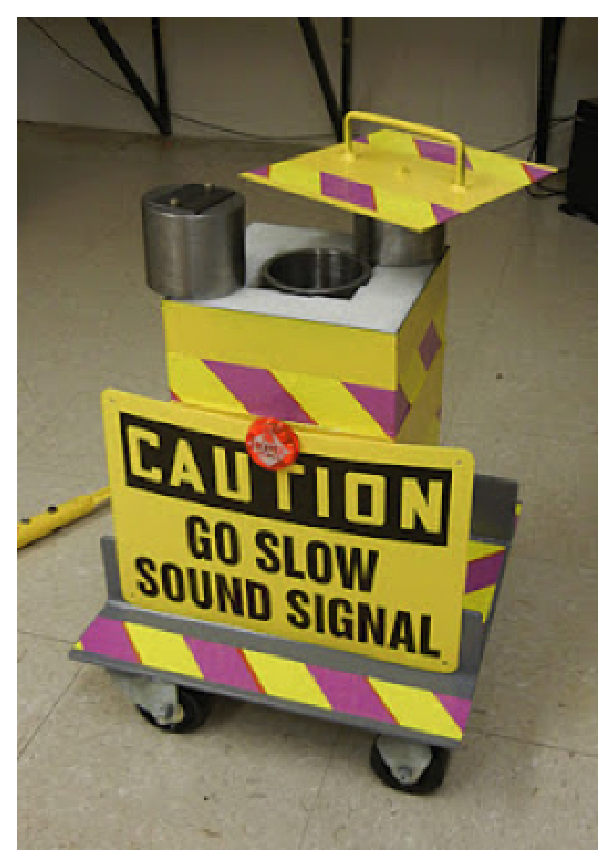
\includegraphics[width=\textwidth]{images/GammaIrridiator.eps}
		\label{fig:GammaIrridiator}
		\caption{Gamma Irridiator}
	\end{figure}
\end{column}
\end{columns}
\end{frame}

\begin{frame}{Neutron Irridiator}
\begin{columns}[onlytextwidth]
\begin{column}{0.45\textwidth}
	text
\end{column}
\begin{column}{0.45\textwidth}
	\begin{figure}
		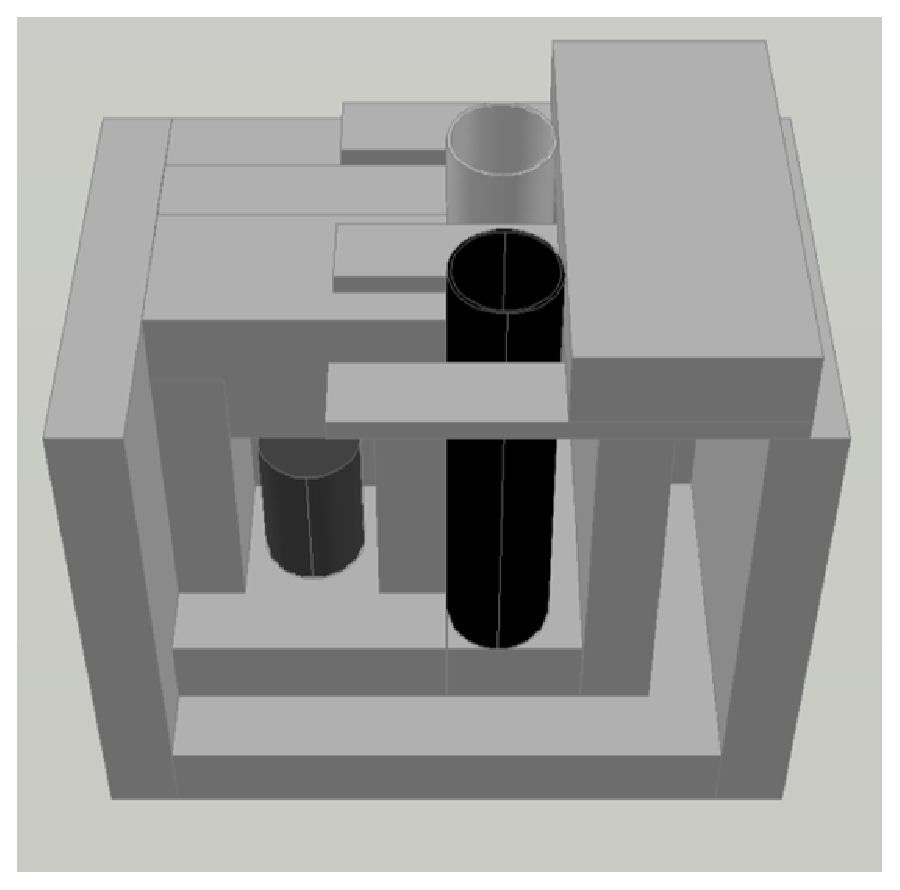
\includegraphics[height=0.25\textheight]{images/NeutronIrridiator_CAD.eps}
		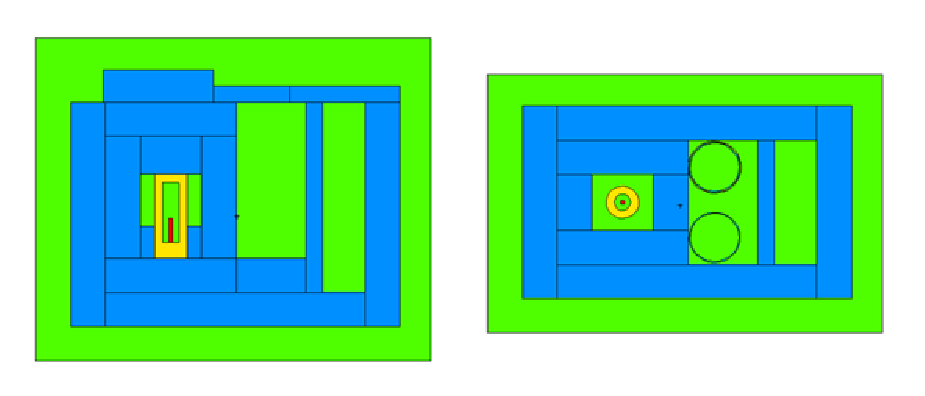
\includegraphics[height=0.25\textheight]{images/NeutronIrridiator_MCNP.eps}
	\end{figure}
\end{column}
\end{columns}
\end{frame}
